\chapter{Referencial teórico}
\label{chp:referencial_teorico}

Como base do conteúdo a ser referenciado dentro deste trabalho, existem diversas tecnologias e conceitos que são de fundamental importância, de modo que seja entendido desde os comparativos das ferramentas a serem expostas e como interagem com o kernel. Assim temos a seguir os conceitos a serem tratados.

\section{Virtualização}
Como início desta sessão, vamos definir virtualização como uma entidade de software da qual representa um recurso real de hardware, mas não necessariamente representando todas as capacidades deste recurso de hardware, como exemplo, digamos que exista um processador que possua 8 núcleos e 16 threads, mas a virtualização deste recurso representa apenas 4 núcleos e 8 threads deste processador real.

Desta forma, temos a virtualização como base do sandbox, sendo este feito através do isolamento de recursos, sejam estes limitações quanto operações, quanto quantidade de recursos.

Portanto, a virtualização, dos recursos funciona como um proxy para o acesso aos recursos de forma real, assim possibilitando os controles e isolamentos previamente citados. Assim sua base gira em torno de um sistema agir de modo intermediário ao hardware e definir quais seriam os recursos que estariam disponíveis para determinado programa ou Sistema Operacional (SO).

A categorização dos tipos de virtualização em alto nível, isto é sem entrar em muitos detalhes conceituais, gira em torno dos tipos de virtualização através de uma máquina virtual (MV) e a conteinerização.

Temos a MV e esta precisa do hypervisor, uma camada de abstração aos recursos reais de hardware a serem providos no sistema. Como exemplo digamos que temos um dispositivo de armazenamento o qual interage diretamente com o hypervisor através de seus drivers, o hypervisor  gera um driver virtual do qual é utilizado dentro da MV para interagir com o SO convidado.

Já na conteinerização, o processo é mais simples por disponibilidade de alguns recursos providos pelo GNU/Linux, os quais são os Namespaces e cgroups, que possibilitam gerenciar acesso e uso de recursos sem utilização de muitas abstrações utilizadas em uma MV (criação de um driver virtual). Além de todos os processos rodarem no mesmo SO, o qual pode ser verificado na máquina host como só mais um processo na árvore de processos, diferentemente de uma MV que aponta a existência de um único processo. Mais a respeito pode ser visto no tópico \ref{chp:referencial_teorico::sct:containers}.

Em questão de comparação entre estes tipos de virtualização, MV e container, temos a seguinte tabela comparativa:

\begin{tabular}{|c|p{5cm}|p{5cm}|}
\hline
\textbf{Parametro} & \textbf{Máquina Virtual} & \textbf{Container} \\
\hline
OS convidado    & Roda sobre hardware virtual e kernel é carregado em sua própria região de memória & Todos os convidados compartilham o mesmo kernel, e a imagem do kernel é carregado na memória física \\
\hline
Comunicação     & Será feita através de dispositivos de rede & Mecanismos padrões de IPC, como sinais, pipes, sockets, etc \\
\hline
Segurança       & Depende da implementação do Hypervisor & Mecanismos de controle do kernel \\
\hline
Performance     & Sofre do overhead das instruções a serem traduzidas do convidado para o host & Provém uma performance quase nativa \\
\hline
Isolamento      & Bibliotecas compartilhadas, arquivos e etc, não podem ser compartilhados entre convidado e host & Subdiretórios podem ser montados e compartilhados entre host e container \\
\hline
Tempo de inicio & Precisam de alguns minutos para iniciar  &  Podem ser iniciados em segundos \\
\hline
Armazenamento  & Precisa de muito armazenamento para seu kernel, programas e dependências &  Ocupam menos espaço uma vez que o kernel é compartilhado \\
\hline
\end{tabular}


\section{Hypervisors}
Em essência é um software especial para virtualização de SOs do qual cuida basicamente de 2 aspectos, a emulação de instruções privilegiadas, as quais apenas o SO instalado diretamente no hardware poderia fazer, e virtualização de dispositivos, estes sendo responsável por hardwares de entrada e saída de dados \cite{kernelscheepers}.

CONSULTAR ARTIGOS SOBRE RINGS DO PROCESSADOR

\section{Máquina Virtual (MV)}
\label{chp:referencial_teorico::sct:maquina_virtual}
O caso da máquina virtual, normalmente é utilizado visando rodar múltiplos SOs diferentes e até de arquiteturas diferentes. Seu uso implica na virtualização de todos os recursos providos pelo hardware e provimento de drivers virtuais para estes SOs. Possuindo em si algumas outras segmentações, tais como a virtualização de tipo 1 (bare-metal) e tipo 2 \cite{kernelscheepers, Virtualization_vs_Containerization}.

Como visualização das diferenças entre os tipos de virtualização providos por MVs, temos a figura \ref{fig:virtualization_t1_vs_t2}.

\begin{figure}
    \centering
    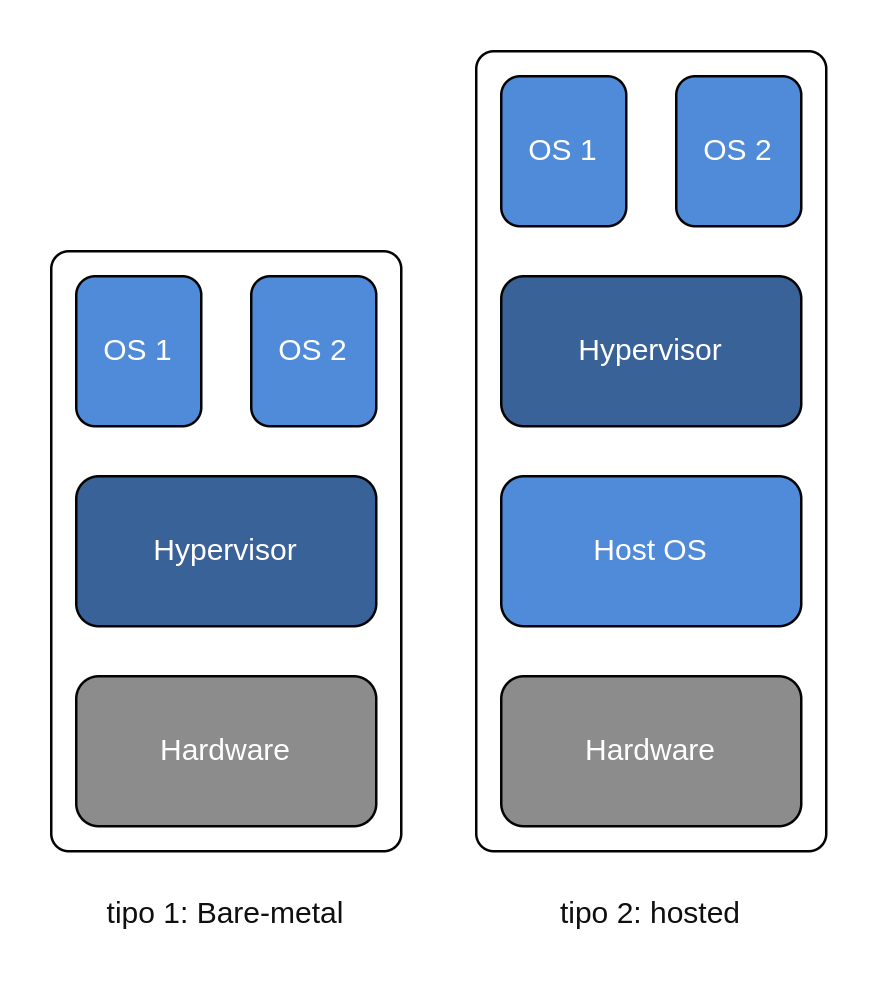
\includegraphics[width=8cm]{images/vm_t1_vs_t2.drawio.png}
    \caption{Virtualização tipo 1 vs tipo 2}
    \label{fig:virtualization_t1_vs_t2}
\end{figure}

\subsection{Tipo 1 - Bare-metal}
No tipo de virtualização bare-metal, temos o hypervisor que cuida de todo o gerenciamento do recurso e distribuição dos mesmos para cada SO convidado. Possuem performance melhor em comparação ao tipo 2, uma vez que seu acesso intercede exclusivamente o hypervisor, assim rodando praticamente de forma nativa.

A respeito deste tipo, o GNU/Linux implementa um módulo kernel-based virtualization machine (KVM), o qual resulta na capacidade de virtualização sobre este funcionar tal como um hypervisor. Deste modo, praticamente qualquer kernel Linux com este módulo pode ser utilizado tal como um hypervisor \cite{what-is-KVM}.

\subsection{Tipo 2 - Hosted Hypervisor}
Já no tipo 2, inicia-se um SO principal, e este através de virtualização de hardware e/ou tradução de interfaces binárias, possibilita o uso de recursos em um SO convidado. A comunicação do SO convidado com os recursos tende a ser mais demorada devido sua comunicação levar seu tempo de interpretação do SO principal, que por fim acessa o recurso solicitado, resultando assim em uma execução mais lenta quando comparado a virtualização tipo 1 bare-metal.

\section{Syscalls - Chamadas de sistema}
\label{chp:referencial_teorico::sct:syscall}
É uma rotina que permite um processo em userland (isto é, qualquer processo que não seja do kernel) requisitar ações permitidas apenas por acessos privilegiados, isto é, uma aplicação sendo executada em nível de usuário solicita ao kernel acessos a funções privilegiadas do kernel, tais como leitura e escrita em arquivos e envio de dados na rede \cite{syscall-ibm, syscall-kerrisk}.

\section{Namespaces}
\label{chp:referencial_teorico::sct:namespace}
A tecnologia consiste em fazer o isolamento dos recursos a serem utilizados por determinado processo. Deste modo o namespaces é uma camada de interação que se encontra entre a execução propriamente dita e sua interação com kernel, tal como um proxy \cite{kernelscheepers}.

Esta camada que se encontra entre o processo e o kernel, atua quando determinado software executa uma Syscall e as estruturas do processo, das quais possuem determinado namespace, delimita quais recursos estão disponíveis para o processo.

Desta forma cria-se uma virtualização dos recursos que estão disponíveis e quais são eles, uma vez que a resposta para o software a ser executada é dada pelas configurações daquele namespaces sobre o qual a aplicação roda. Sendo esta a base para criação de containers, a limitação dos recursos, dos quais trata-se de um processo, o qual roda de maneira isolada em um SO.

Por fim, uma vez compreendida sua função, é necessário a compreensão de quais tipos de namespaces estão disponíveis uma vez que utilize-se o kernel GNU/Linux.

\begin{itemize}
    \item \textbf{mnt}: Pontos de montagem no sistema.
    \item \textbf{PID}: Id de processo.
    \item \textbf{net}: Stack de rede.
    \item \textbf{IPC}: Comunicação entre processos.
    \item \textbf{usr}: Usuário de sistema.
    \item \textbf{UTS}: Unix Timesharing System, para sincronização entre processos independente.
\end{itemize}

Sendo então estes os namespaces que existem na atualidade para fazer o isolamento de determinado processo aos recursos que são disponibilizados pela kernel.

\section{Cgroups}
\label{chp:referencial_teorico::sct:cgroup}
O controle de grupos, também chamado de cgroups, é a ferramenta para controle de uso do recurso, sendo esses de alguns tipos diferentes, mas em seu cerne trata-se de controle de quantidade de uso deste, ou seja quanto tempo ou banda de utilização de determinado recurso estaria liberado para um determinado processo do qual se encontra sob aquele cgroup \cite{kernelscheepers, secrypt22}.

Compreendido que se trata do uso de recurso, aqueles que estão sob controle de determinado grupo, pode-se limitar o uso da CPU e utilização de blocos de I/O (entrada e saída de dados). Deste modo, determina-se quanto tempo de processamento está disponível e/ou quantos bytes estão disponíveis na entrada e saída do processo, seja ela utilização de rede (internet), escrita e leitura de arquivos, etc.

\section{Containers}
\label{chp:referencial_teorico::sct:containers}
Os containers, basicamente utilizam recursos supracitados, para fazer o isolamento daquilo que seria disponível para o processo, em geral tratando-se de uma camada a qual não tem acesso irrestrito a recursos do SO, tais como pontos de montagem de arquivos, comunicação entre processos e entre outras funcionalidades \cite{what-container, what-are-container}.

Entretanto vale ressaltar que o processo roda isolado na percepção de si próprio, mas não da SO host do container, do qual tem livre acesso a tudo do processo dentro do container. Isto deve-se a questão deste estar rodando sob o SO host de forma nativa, diferentemente do que ocorre em MVs, resultando assim em inicialização do container de forma imediata.

Como visualização das diferenças entre os tipos de virtualização desde MVs a containers, temos a figura \ref{fig:container_vs_virt_t1_vs_virt_t2}.

\begin{figure}
    \centering
    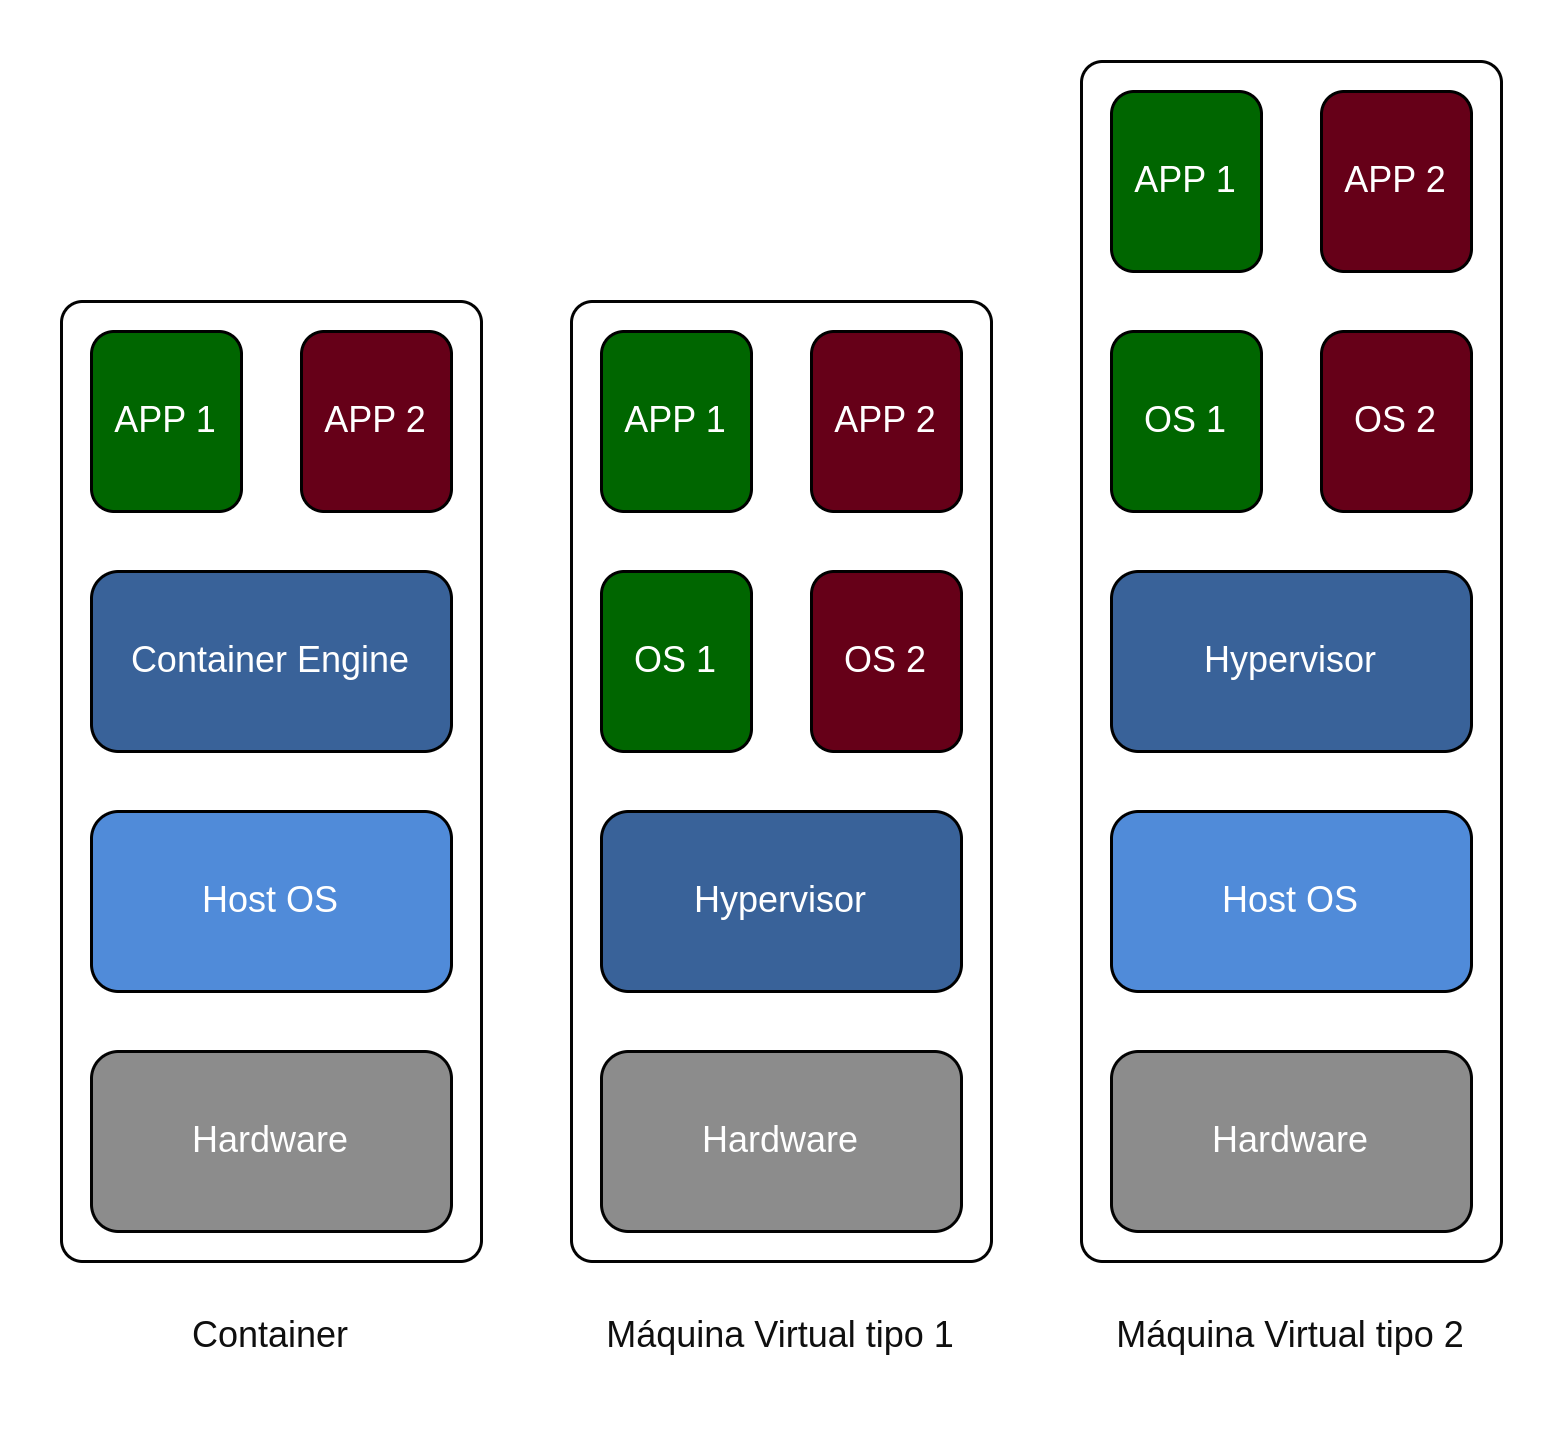
\includegraphics[width=12cm]{images/virt_container_vs_t1_vs_t2.drawio.png}
    \caption{Container vs Virtualização tipo 1 vs tipo 2}
    \label{fig:container_vs_virt_t1_vs_virt_t2}
\end{figure}

